\documentclass{beamer}
\usepackage{listings}
\lstset{
%language=C,
frame=single, 
breaklines=true,
columns=fullflexible
}
\usepackage{subcaption}
\usepackage{url}
\usepackage{tikz}
\usepackage{tkz-euclide} % loads  TikZ and tkz-base
%\usetkzobj{all}
\usetikzlibrary{calc,math}
\usepackage{float}
\newcommand\norm[1]{\left\lVert#1\right\rVert}
\providecommand{\pr}[1]{\ensuremath{\Pr\left(#1\right)}}
\providecommand{\sbrak}[1]{\ensuremath{{}\left[#1\right]}}
\providecommand{\brak}[1]{\ensuremath{\left(#1\right)}}
\providecommand{\fourier}{\overset{\mathcal{F}}{ \rightleftharpoons}}
\providecommand{\ztrans}{\overset{\mathcal{Z}}{ \rightleftharpoons}}
\providecommand{\abs}[1]{\left\vert#1\right\vert}
\renewcommand{\vec}[1]{\mathbf{#1}}
\usepackage[export]{adjustbox}
\usepackage[utf8]{inputenc}
\usepackage{amsmath}
\usetheme{Boadilla}

\title{GATE EC 2010- Q.42}
\author{Tanmay Goyal - AI20BTECH11021}

\date{}

\begin{document}

\begin{frame}
\titlepage
\end{frame}
\begin{frame}
\frametitle{Question}
\begin{flushleft}
The transfer function for a discrete time LTI system is given by:
\begin{align}
    H(z) = \frac{2 - \frac{3}{4}z^{-1}}{1 - \frac{3}{4}z^{-1} + \frac{1}{8}z^{-2}}
\end{align}
Consider the following statements:\\
S1: The system is stable and causal for ROC: $\abs{z} > \frac{1}{2}$\\
S2: The system is stable but not causal for ROC:  $\abs{z} < \frac{1}{4}$\\
S3: The system is neither stable nor causal for ROC:  $\frac{1}{4}<\abs{z} < \frac{1}{2}$\\
Which one of the following statement are valid?
\begin{enumerate}
    \item Both S1 and S2 are true
    \item Both S2 and S3 are true
    \item Both S1 and S3 are true
    \item S1, S2 and S3 are all true
\end{enumerate}
\end{flushleft}
\end{frame}

\begin{frame}[fragile]
\frametitle{Stable and Causal Systems}

\begin{flushleft}
\begin{definition}
We say that a system is \textbf{stable} if it produces a bounded output for every possible bounded input, i.e it satisfies the BIBO(Bounded-input-Bounded-output) condition.
\end{definition}
          \end{flushleft}
    \begin{flushleft}
    \begin{definition}
We say that a system is \textbf{Causal} if the output of a system at a given time instance is independent of the future input values, i.e the output at a particular instance only depends on the present and past input values.

\end{definition}
\end{flushleft}
\end{frame}


\begin{frame}[fragile]
\frametitle{Lemma}
\begin{flushleft}
\begin{lemma}
A system is said to be BIBO stable if and only if the ROC consists of the unit circle in the $Z$ plane.
\end{lemma}
\end{flushleft}

\end{frame}


\begin{frame}[fragile]
\frametitle{Lemma}
\begin{flushleft}
\begin{lemma}
A system is causal if and only if the transfer function $h[n]$ satisfies $h[n] = 0 , n<0$
\end{lemma}
\begin{proof}
Let the input signal be given by $x[n]$ and the output signal be given by $y[n]$, then, we know in an LTI system:
\begin{align}
    y[n] = h[n] * x[n] = \sum_{k = -\infty}^\infty h[k]x[n-k]
\end{align}
Since, $y[n]$ is causal, it should be independent of future values of $n$. \\
If $k < 0$, then $n - k > n$, which is undesirable, and thus, to keep $y[n]$ independent of future values, $h[k] = 0 , k< 0$
\end{proof}
\end{flushleft}

\end{frame}

\begin{frame}[fragile]
\frametitle{Z-transform Lemma}
\begin{flushleft}
\begin{lemma}
If $x[n] = a^nu[n]$, where 
\begin{align}
    u[n] = 
    \begin{cases}
    1 & n \geq 0\\
    0 & otherwise
    \end{cases}
\end{align}
then $x[n] \ztrans X[z] = \frac{1}{1 - az^{-1}}$ with ROC = $\abs{z}>a$
\label{z-transform}
\end{lemma}
\end{flushleft}

\end{frame}

\begin{frame}[fragile]
\frametitle{Z-transform Lemma proof}
\begin{flushleft}
\begin{proof}
Using the formula for the sum of an infinite GP, we get:
\begin{align}
    x[n] = 
    \begin{cases}
    a^n & n\geq 0\\
    0 & otherwise
    \end{cases}\\
    \mathcal{Z}\{x[n]\} = X[z] = \sum_{n = -\infty}^\infty x[n]z^{-n}\\
    = \sum_{n = -\infty}^0 0 \times z^{-n} + \sum_{n = 0}^{\infty} (az^{-1})^n\\
     = \frac{1}{1 - az^{-1}} , ROC = \abs{az^{-1}} < 1\\
      = \frac{1}{1 - az^{-1}} , ROC =  \abs{z} > a
\end{align}
\end{proof}
\end{flushleft}

\end{frame}


\begin{frame}[fragile]
\frametitle{Z-transform Lemma when ROC condition is violated}
\begin{flushleft}
\begin{lemma}
If 
\begin{align}
    X[z] = \frac{1}{1 - az^{-1}}
\end{align} and the region of convergence is
\begin{align}
    Z \setminus (ROC \cup \abs{a})
\end{align} where $Z$ is the entire Z plane and $ROC$ is the region of convergence mentioned in \eqref{z-transform}, then
\begin{align}
    x[n] = -a^nu[-n-1]
\end{align}
\label{ROC-violation}
\end{lemma}
\end{flushleft}
\end{frame}


\begin{frame}{fragile}
\frametitle{Proof}

\begin{flushleft}
\begin{proof}
ROC =  $Z \setminus (ROC \cup \abs{a}) \implies \abs{z}  < \abs{a}$. From \eqref{z-transform}, we see that we cannot apply the formula for the sum of an infinite GP directly as the conditions are not satisfied. Thus, we manipulate the function.
\begin{align}
    \abs{z}  < \abs{a} \implies \abs{\frac{z}{a}} < 1\\
    \frac{1}{1 - az^{-1}} = \frac{-z}{a}\frac{1}{1 - \frac{z}{a}} , \abs{\frac{z}{a}} < 1\\
     = \sum_{n = 0}^\infty \frac{-z}{a} \brak{\frac{z}{a}}^n\\
     = - \sum_{n = 0}^\infty  \brak{\frac{z}{a}}^{n+1}\\
       = - \sum_{n = -\infty}^\infty  \brak{\frac{z}{a}}^{n+1}u[n]\\
\end{align}
\end{proof}
\end{flushleft}

\end{frame}
\begin{frame}{fragile}
\frametitle{Proof continued}

\begin{flushleft}
\begin{proof}
\begin{align}
    = -\sum_{n = -\infty}^\infty  a^{-n-1}z^{n+1}u[n]\\
      = -\sum_{k = -\infty}^\infty  a^{k}z^{-k}u[-k-1]
\end{align}
by substituting $n+1 = -k$\\
Finally, on comparing with the general z-transform formula of $x[n] \ztrans X[z] = \sum_{n = -\infty}^\infty x[n]z^{-n}$, we get:
\begin{align}
    x[n] = -a^nu[-n-1]
    \end{align}
\end{proof}
\end{flushleft}
\end{frame}

\begin{frame}
    \frametitle{Decomposition of Transform Function}
    \begin{flushleft}
     We are given the transfer function:
\begin{align}
    H(z) = \frac{2 - \frac{3}{4}z^{-1}}{1 - \frac{3}{4}z^{-1} + \frac{1}{8}z^{-2}}
\end{align}
To find the inverse Z-Transform, we would decompose the function using partial fractions:
\begin{align}
    H(z) = \frac{16 - 6z^{-1}}{8 - 6z^{-1} + z^{-2}}\\
     = \frac{16 - 6z^{-1}}{(4 - z^{-1})(2 - {z^{-1}})}\\
      = \frac{4}{4 - z^{-1}} +\frac{2}{2 - z^{-1}}\\
       = \frac{1}{1 - \frac{1}{4}z^{-1}} + \frac{1}{1 - \frac{1}{2}z^{-1}}
       \label{partial-fraction}
\end{align}
  \end{flushleft}
\end{frame}

\begin{frame}
    \frametitle{When ROC: $\abs{z} > \frac{1}{2}$}
    \begin{flushleft}
   If ROC = $\abs{z}>\frac{1}{2}$, this automatically implies $\abs{z} > \frac{1}{4}$, thus, from \eqref{z-transform}, we can say:
\begin{align}
    h[n] = \brak{\frac{1}{2}}^n u[n] + \brak{\frac{1}{4}}^n u[n] 
\end{align}
Since ROC = $\abs{z}>\frac{1}{2}$ includes the unit circle, the system is stable.\\
Moreover, we see $h[n] = 0 $
 for $n < 0$, since $u[n] = 0$ for $n< 0$. Thus, the system is Causal as well.\\\textbf{Hence, S1 is correct}\\
    \end{flushleft}
\end{frame}

\begin{frame}
    \frametitle{When ROC: $\abs{z} > \frac{1}{2}$}
    \begin{flushleft}
   \begin{figure}[!ht]
\centering
 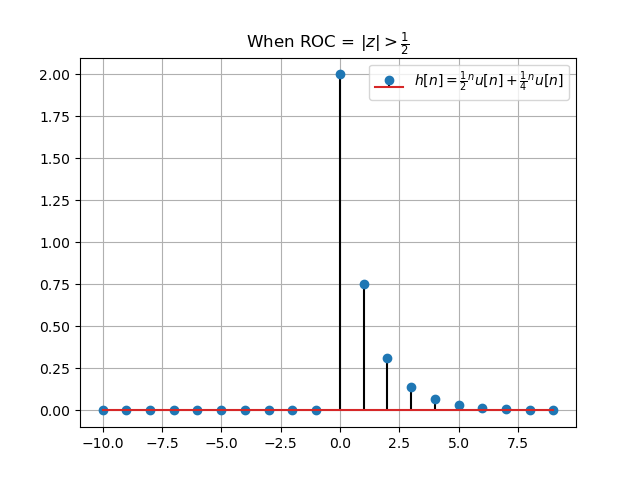
\includegraphics[width=\columnwidth]{graphs/S1.png}
 \caption{$h[n]$ when $\abs{z} > \frac{1}{2}$}
 \end{figure}    \end{flushleft}
\end{frame}

\begin{frame}
    \frametitle{When ROC = $\frac{1}{4} < \abs{z} < \frac{1}{2}$}
    \begin{flushleft}
    Since the unit circle is not included in the ROC, the system cannot be stable. Moreover, the ROC condition for only one of the two fractions in \eqref{partial-fraction} is satisfied, i.e
 \begin{align}
     \brak{\frac{1}{4}}^nu[n]\ztrans \frac{1}{1 - \frac{1}{4}z^{-1}}  , \abs{z} > \frac{1}{4}
 \end{align}
 Since, the ROC condition is not satisfied for the other term, from \eqref{ROC-violation}, we get:
 \begin{align}
    -\brak{\frac{1}{2}}^nu[-n-1] \ztrans \frac{1}{1 - \frac{1}{2}z^{-1}} , \abs{z} < \frac{1}{2}
 \end{align}
    \end{flushleft}
\end{frame}

\begin{frame}
    \frametitle{When ROC = $\frac{1}{4} < \abs{z} < \frac{1}{2}$ continued}
    \begin{flushleft}
   Thus, for the ROC = $\frac{1}{4} < \abs{z} < \frac{1}{2}$, we get:
 \begin{align}
     h[n] = \brak{\frac{1}{4}}^nu[n]  -\brak{\frac{1}{2}}^{n} u[-n-1] 
 \end{align}
 Clearly, for $n<-1$ , $-n-1 > 0$ and hence, $h[n] \neq 0$ for $n<0$, and thus, the system is non-causal.\\
\textbf{S3 is also correct}.\\
    \end{flushleft}
\end{frame}

\begin{frame}
    \frametitle{When ROC = $\frac{1}{4} < \abs{z} < \frac{1}{2}$}
    \begin{flushleft}
    \begin{figure}[!ht]
\centering
 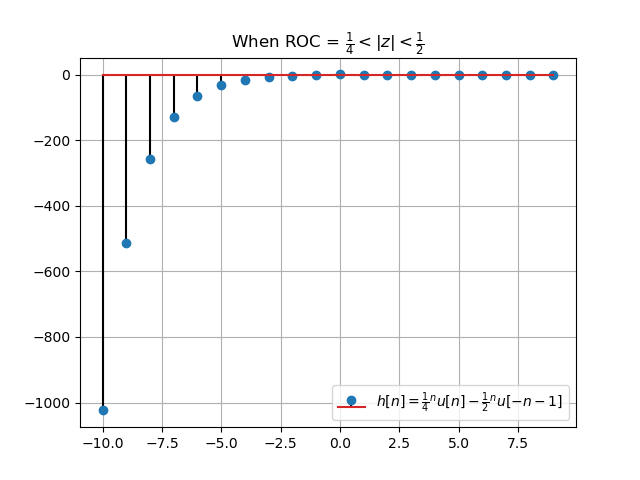
\includegraphics[width=\columnwidth]{graphs/S3.png}
 \caption{$h[n]$ when $\frac{1}{4}<\abs{z} < \frac{1}{2}$}
 \end{figure}
    \end{flushleft}
\end{frame}


\begin{frame}
    \frametitle{When ROC = $\abs{z} < \frac{1}{4}$}
    \begin{flushleft}
    this automatically implies $\abs{z} < \frac{1}{2}$. Since the unit circle is not included, the system is unstable. Moreover, from \eqref{z-transform}, since both the ROC conditions are violated, from \eqref{ROC-violation}, we get:
\begin{align}
    -\brak{\frac{1}{2}}^nu[-n-1] \ztrans \frac{1}{1 - \frac{1}{2}z^{-1}} , \abs{z} < \frac{1}{2}\\
    -\brak{\frac{1}{4}}^nu[-n-1] \ztrans \frac{1}{1 - \frac{1}{4}z^{-1}} , \abs{z} < \frac{1}{4}
\end{align}
Thus, we get:
\begin{align}
    h[n] = -\brak{\frac{1}{2}}^nu[-n-1] -\brak{\frac{1}{4}}^nu[-n-1]\\
    h[n] = -u[-n-1]\sbrak{\brak{\frac{1}{2}}^n + \brak{\frac{1}{4}}^n}
\end{align}
Clearly, for $n<-1$ , $-n-1 > 0$, and thus, $h[n] \neq 0 , n<0$. The system is non-causal.
\textbf{Hence, S2 is incorrect}\\
   \end{flushleft}
\end{frame}

\begin{frame}
    \frametitle{When ROC = $\abs{z} < \frac{1}{4}$}
    \begin{flushleft}
      \begin{figure}[!ht]
\centering
 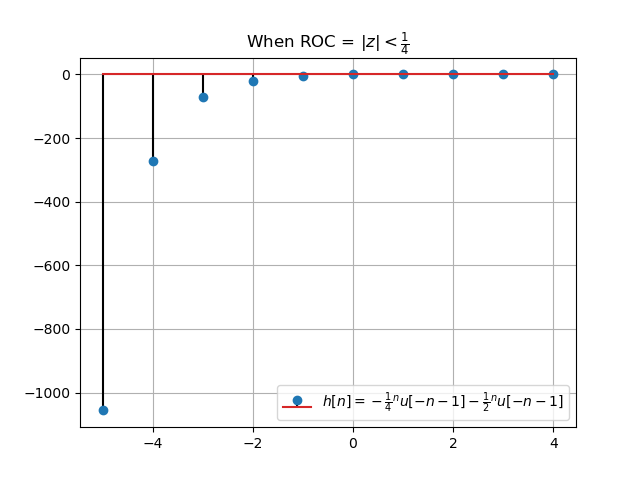
\includegraphics[width=\columnwidth]{graphs/S2.png}
 \caption{$h[n]$ when $\abs{z} < \frac{1}{4}$}
 \end{figure}
   \end{flushleft}
\end{frame}


\begin{frame}
    \frametitle {ROC}
    \begin{flushleft}
    \begin{figure}[!ht]
\centering
 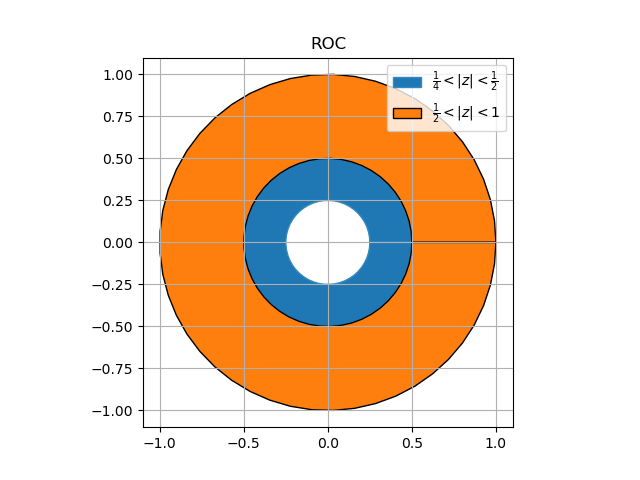
\includegraphics[width=\columnwidth]{graphs/ROC.png}
 \caption{ROC}
 \end{figure}
    \end{flushleft}
\end{frame}

\end{document}